To determine the beam density at the trap, we characterize the rate at which \ce{Be+} reacts with water from the beam. \ce{Be+} nad \ce{C+} are loaded into the ion trap and laser cooled until a cloud or crystal forms, then the trap region is exposed to the CBGB with entrained \ce{H2O}. The reaction products are ejected from the trap into the time of flight mass spectrometer (TOF-MS) at various delay times and the integrated ion signal is recorded. Assuming a forward velocity for \ce{H2O} upwards of 200 m/s, we have a reaction temperature of $\approx$20 K. The interaction produces reactions \ref{r: Be(S)+H2O->BeOH} and \ref{r: Be(P)+H2O->BeOH}, which were experimentally determined to react at temperature ($T$) and \ce{^2P3/2} state excitation fraction ($P$) at a rate defined by equation \ref{eq: k Be+H2O(T)}.

\begin{figure}[H]
	\centering
	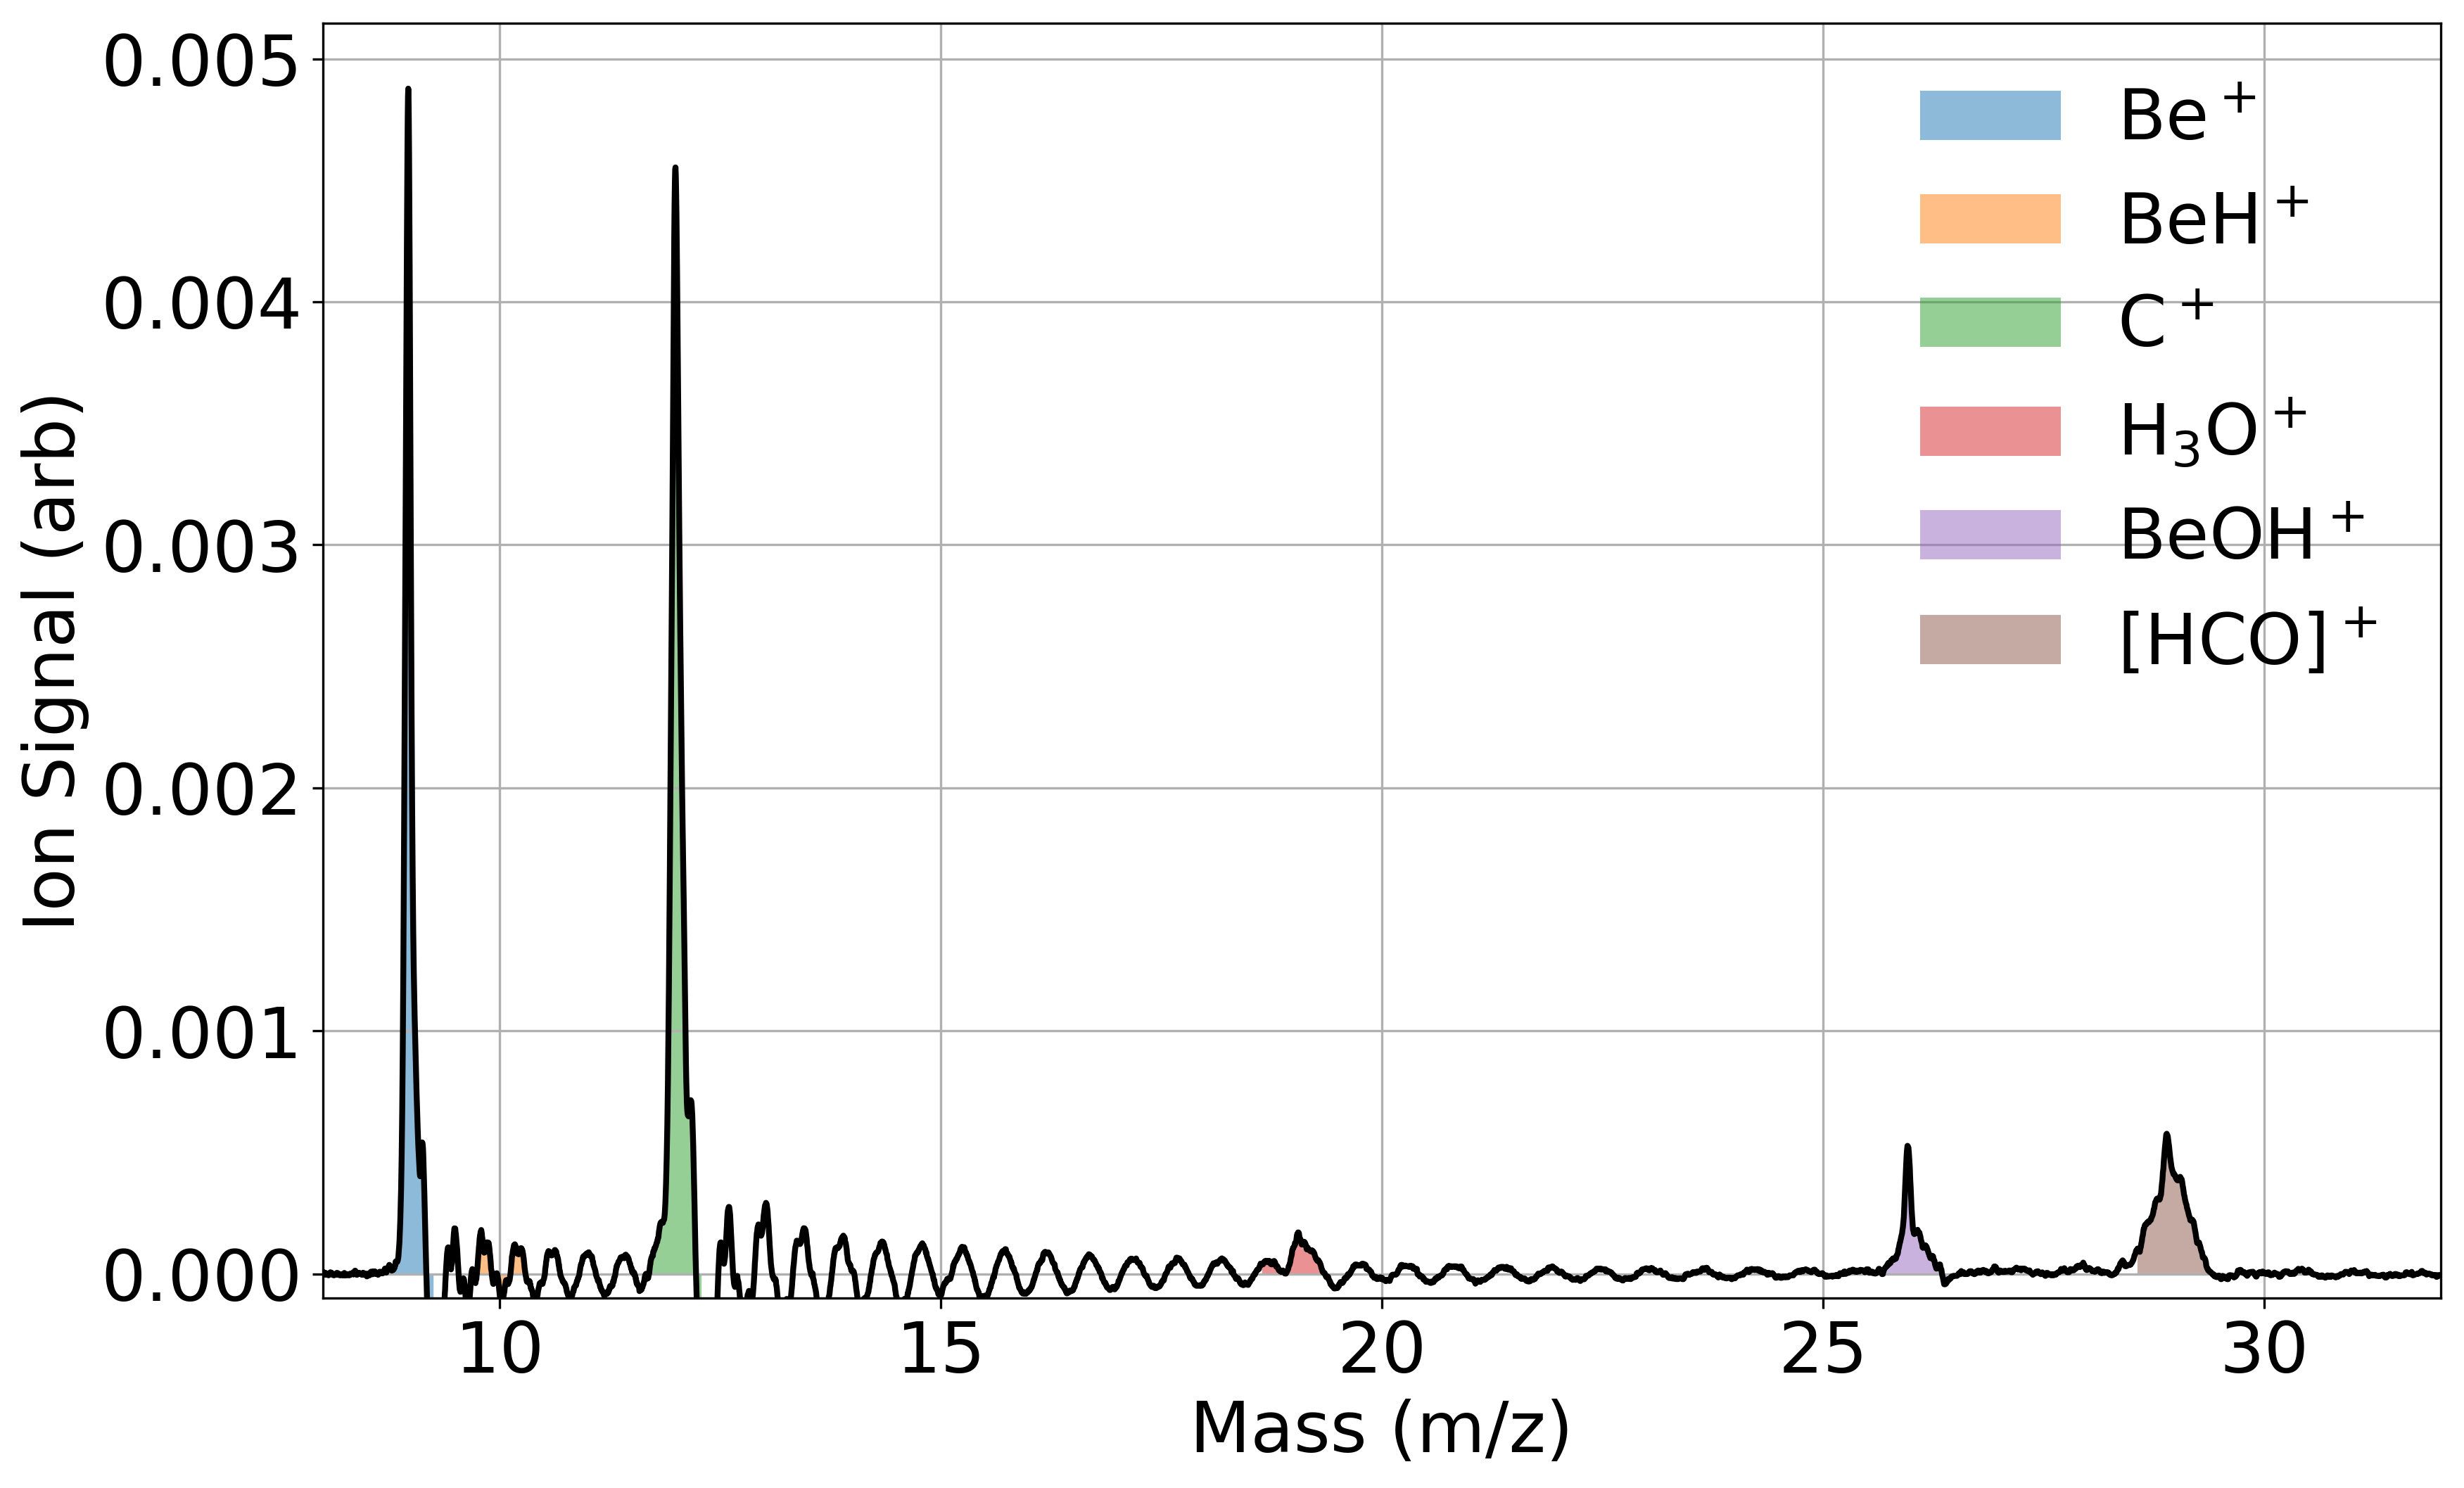
\includegraphics[width=0.8\textwidth]{images/C_H2O_beam_TOF.png}
	\caption{text}
	\label{fig: Be C H2O beam TOF}
\end{figure}

\begin{figure}[H]
	\centering
	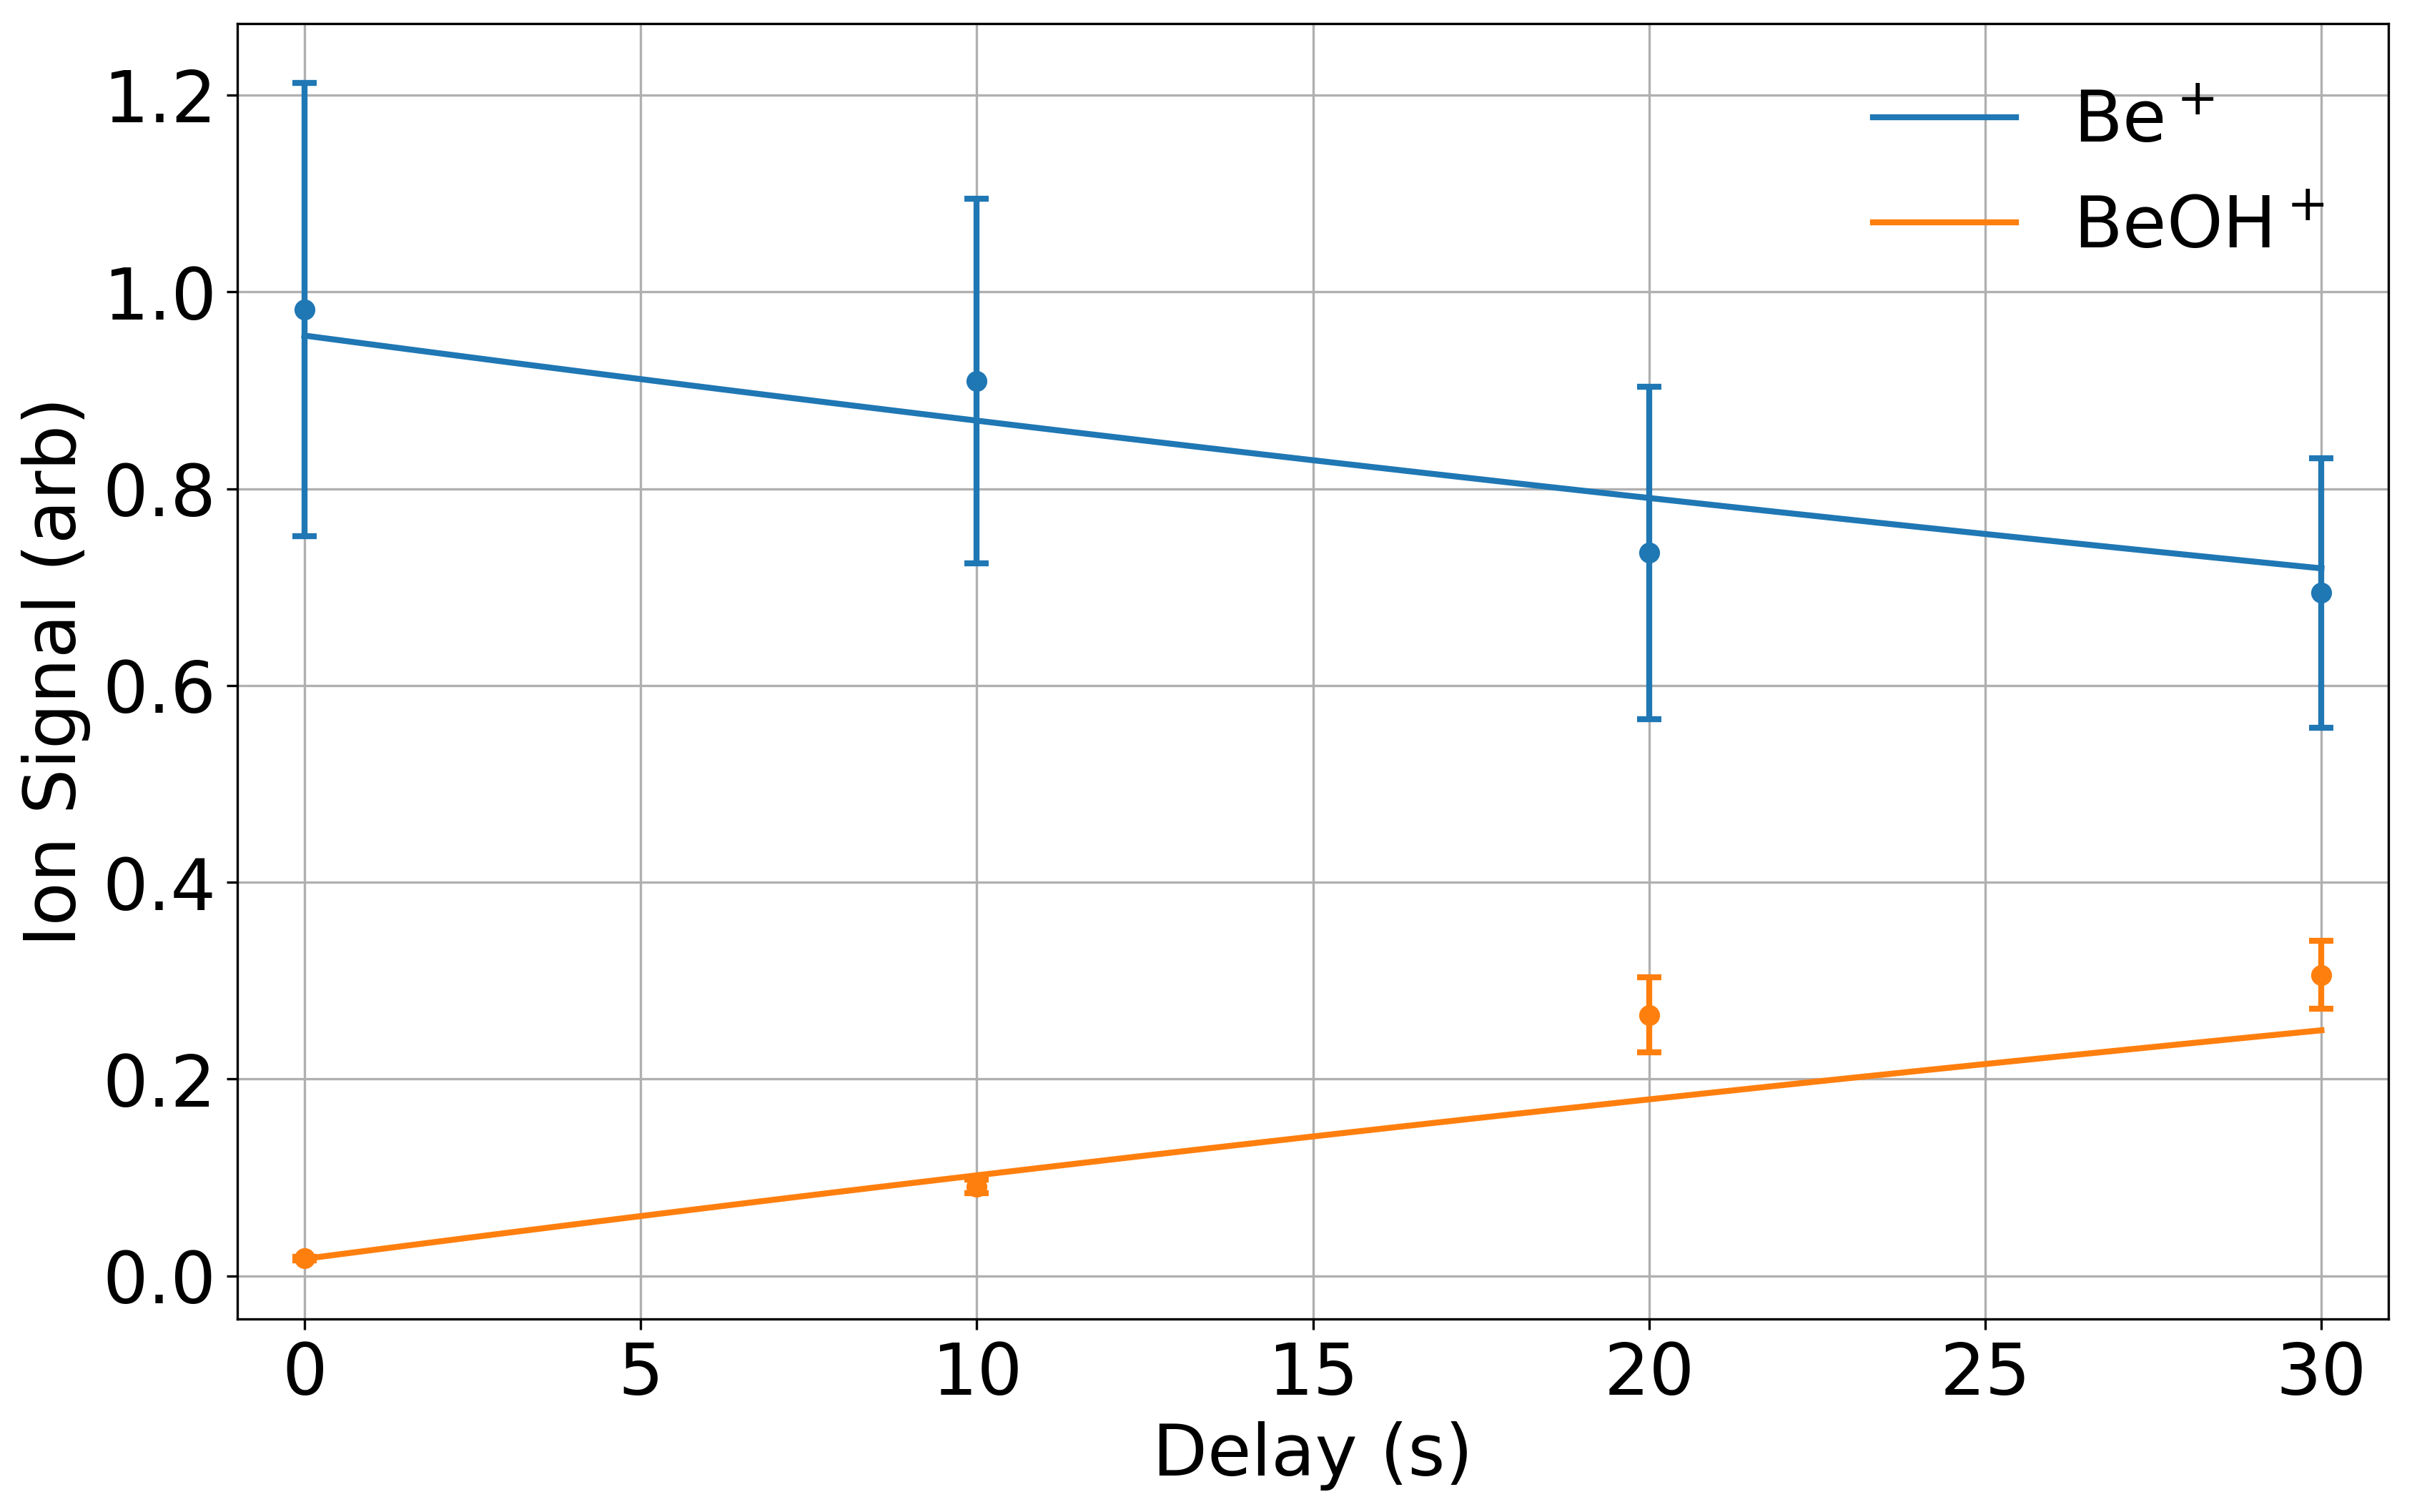
\includegraphics[width=0.8\textwidth]{images/Be_H2O_beam_traces.png}
	\caption{\ce{Be+} decay and \ce{BeOH+} appearance due to the introduction of \ce{H2O} from the CBGB. A shared fit of rates \ref{r: Be(S)+H2O->BeOH} and \ref{r: Be(P)+H2O->BeOH} yields a water beam density $\rho_{beam} = (2.18 \pm 0.37) \times 10^6$ cm$^{-3}$.}
%	Reduced chi square of 2
	\label{fig: Be H2O beam}
\end{figure}

Using the ADO approximation